\documentclass{scrartcl}

\usepackage{
  calc,
  cooltooltips,
  dtklogos,
  filecontents,
  geometry,
  graphicx,
  hyperref,
  lmodern,
  natbib,
  tikz
}

\geometry{
%  landscape,
  margin=1cm
}
\hypersetup{
  colorlinks=true,
  linkcolor=blue,
  urlcolor=blue,
  pdfborder=0 0 0
}

\def\XeT{XET}
\def\Aleph{Aleph}
\def\XeLaTeX{Xe\LaTeX}
\def\ConTeXt{Con\TeX{}t}
%\setmainfont{Linux Libertine}

\def\mynode#1#2#3#4{
  \node (#1) at (#2) {
    \cooltooltip{#1}{#3}{#3}{}{#4\strut}
  };
  \expandafter\def\csname texname#1\endcsname{#3}
  \AtEndDocument{\subsubsection*{\color{blue}#4}\parbox{\textwidth}{#3}}
}

\newlength{\layer}\setlength{\layer}{0cm}
\def\setlayer#1{\setlength{\layer}{#1cm}}
\newcommand\steplayer[1][-1]{\addtolength{\layer}{#1cm}}%\addtocounter{layer}{#1}}

\title{A short overview of \TeX\ and its children \dots}
\author{Arno Trautmann\thanks{arno.trautmann@gmx.de -- Please feel free to mail me any suggestions and comments!}}
\date{}
\pagestyle{empty}

\def\overviewsection#1{\section{#1}\AtEndDocument{\section{#1}}}

\begin{document}
\maketitle

\begin{abstract}
This paper tries to give a short overview of the development of \TeX. The base frame is taken from the article \textsf{A brief history of \TeX, volume II} by Arthur Reutenauer in the proceedings of \textsf{EuroBacho\TeX 2007} and his talk there (see references). Additional information is taken from documentations (see references on page \pageref{sec:refs}). All information is up to the date of the generated pdf. Everything here is without guarantee -- this is just to get an overview. Consult the references for further (and/or correct) information!
\end{abstract}

\tableofcontents

\clearpage
\part{Tree Views}
\newpage
\overviewsection{\TeX\ -- the program, and extensions/derivatives}
\Large
\centering
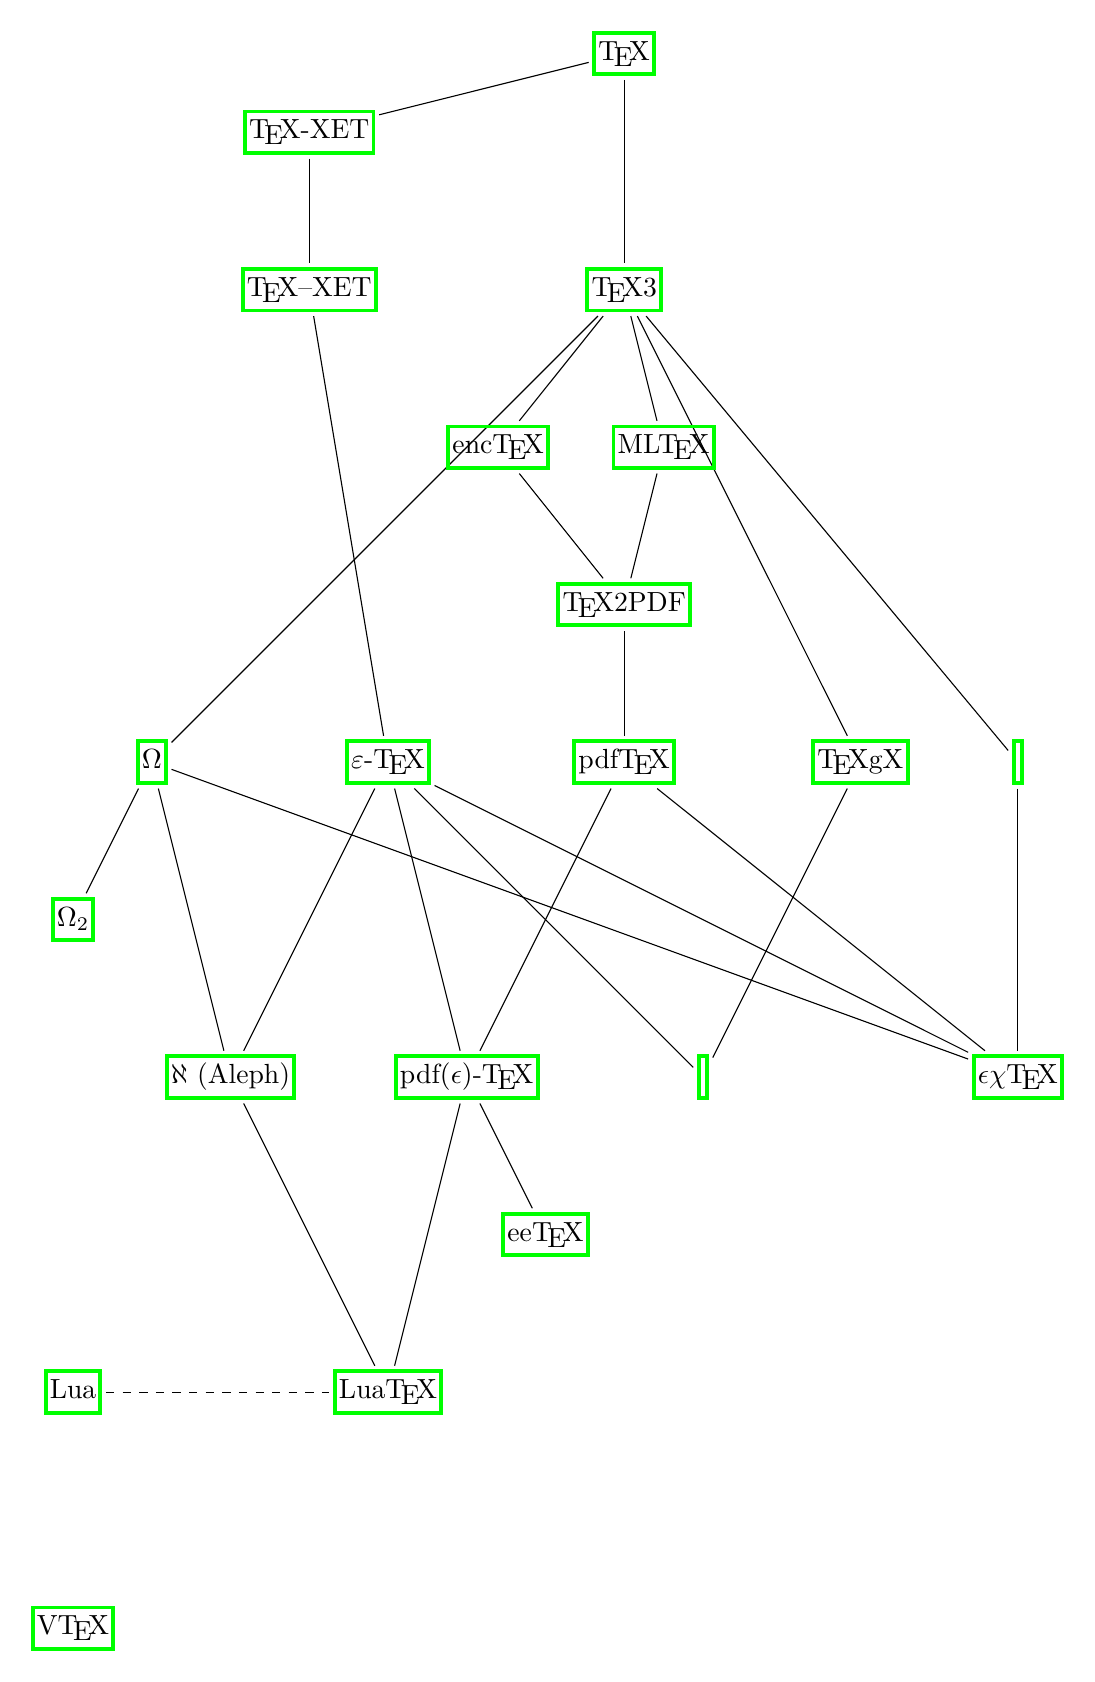
\begin{tikzpicture}
\setlayer2
\mynode{tex}{7,\layer}{born in 1978}{\TeX}

\steplayer
\mynode{xet-tex}{3,\layer}{The first extension to TeX, 1987. It was able to typeset in two directions, but only with a mark in the dvi to change the direction.}{\TeX-\XeT}
\draw (tex) to (xet-tex);

\steplayer[-2]
\mynode{xet--tex}{3,\layer}{TeX--XeT was able to really put the glyphs on the right place in the dvi.}{\TeX-{}-\XeT}
\draw (xet-tex) to (xet--tex);

\mynode{tex3}{7,\layer}{Ability to handle 8-bit input. 1989. TeX development was frozen in 1991.}{\TeX3};
\draw (tex) to (tex3);

\steplayer[-2]
\mynode{enctex}{5.4,\layer}{A small extension to TeX, started 1997. Adds 10 new primitives relating input re-encoding}{enc\TeX};
\draw (tex3) to (enctex);

\mynode{mltex}{7.5,\layer}{Extension (started 1990) to TeX that allows hyphenation of words with accented letters. Distributed as a change file to the original WEB sources of TeX.}{ML\TeX};
\draw (tex3) to (mltex);

\steplayer[-2]
\mynode{tex2pdf}{7,\layer}{Early name for pdfTeX.}{\TeX2PDF};
\draw (enctex) to (tex2pdf);
\draw (mltex) to (tex2pdf);

\steplayer[-2]
\mynode{omega}{1,\layer}{Support for unicode-input. Still constrained on the output}{$\Omega$};
\draw (tex3) to (omega);

\mynode{etex}{4,\layer}{*the* extension to TeX.}{$\varepsilon$-\TeX};
\draw (xet--tex) to (etex);

\mynode{pdftex}{7,\layer}{A new engine to directly produce pdf-files from TeX, without the need of dvi-ps-pdf. This allows to use microtypographic extensions and many other features of the pdf format.}{pdf\TeX};
\draw (tex2pdf) to (pdftex);

\mynode{texgx}{10,\layer}{?}{\TeX{}gX};
\draw (tex3) to (texgx);

\mynode{nts}{12,\layer}{A project to completely reimplement TeX in Java. Now NTS is officially declared dead.}{\NTS};
\draw (tex3) to (nts);

\steplayer[-2]
\mynode{omega2}{0,\layer}{A short-time try to pick up the development of Omega again in 2006. Seemed more like a good plan and is now regarded as obsolete. LuaTeX is kind of a successor.}{$\Omega_2$};
\draw (omega) to (omega2);

\steplayer[-2]
\mynode{aleph}{2,\layer}{originally named epsilon-Omega, an attempt to stabilize Omega while merging epsilon extensions.}{$\aleph$ (\Aleph)};
\draw (omega) to (aleph);
\draw (etex) to (aleph);

\mynode{xetex}{8,\layer}{This extension enables full multilingual support for left-to-right typesetting, right-to-left and almost any other possible direction. XeTeX also features support for OpenType and AAT-fonts.}{\XeTeX};
\draw (texgx) to (xetex);
\draw (etex) to (xetex);

\mynode{extex}{12,\layer}{Planned implementation of a high-quality typesetting system, written in Java. Based on experiences in NTS, eTeX, pdfTeX and Omega. Started in 2003, current version in repository is 0.0. (i. e. not very far ...)}{$\epsilon\chi$\TeX};
\draw (nts) to (extex);
\draw (omega) to (extex);
\draw (etex) to (extex);
\draw (pdftex) to (extex);

\mynode{pdfetex}{5,\layer}{Merging the pdfTeX engine with the eTeX-extensions. This engine can produce dvi (with or without the eTeX-extensions) as well as pdf (again, with or without extensions).}{pdf($\epsilon$)-\TeX};
\draw (etex) to (pdfetex);
\draw (pdftex) to (pdfetex);

\steplayer[-2]
\mynode{eetex}{6,\layer}{Experimental extension to pdfeTeX by Taco Hoekwater, created 2000. Distributed as change file.}{ee\TeX};
\draw (pdfetex) to (eetex);

\steplayer[-2]
\mynode{lua}{0,\layer}{Script language; has nothing to do with TeX!}{Lua};

\mynode{luatex}{4,\layer}{Still in heavy active development, LuaTeX will support unicode, OpenType and totally everything. It features an embedded scripting language, lua, making it easy to extend.}{Lua\TeX};
\draw (aleph) to (luatex);
\draw (pdfetex) to (luatex);
\draw[dashed] (lua) to (luatex);

\steplayer[-3]
\mynode{vtex}{0,\layer}{Please insert information here ...}{V\TeX};
\end{tikzpicture}


\newpage
\overviewsection{\LaTeX\ (Lamport's \TeX) -- a format and large macro package for \TeX}
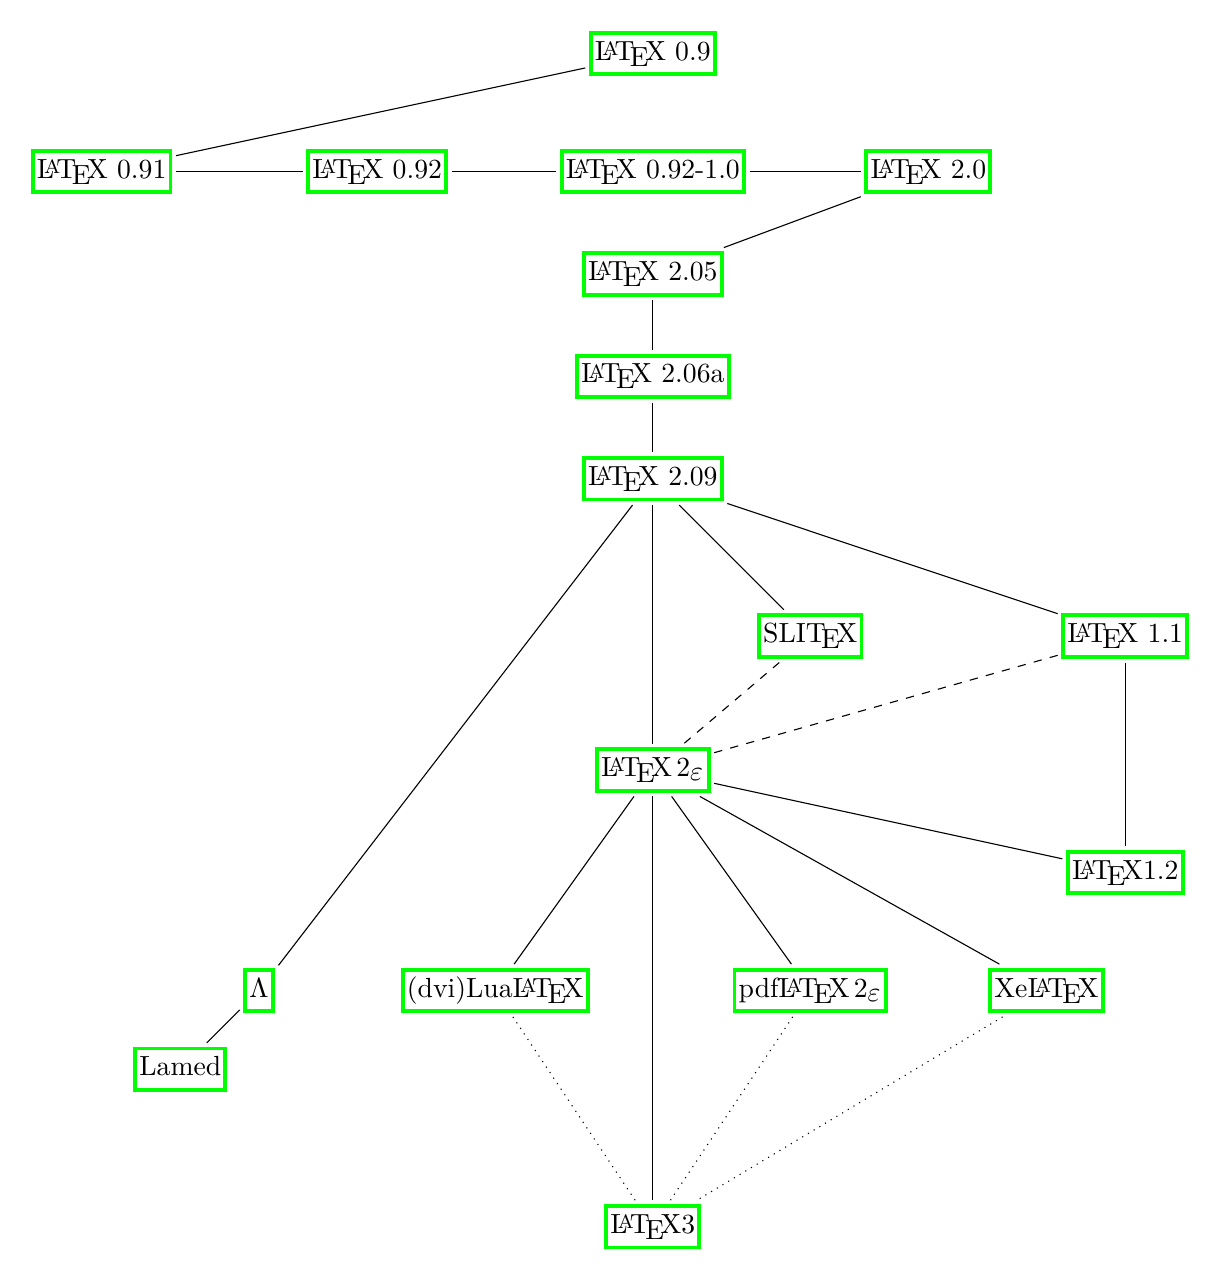
\begin{tikzpicture}
\setlayer{2}
\mynode{latex090}{0,\layer}{First version still on web (historic archive, see refs) is 0.9, for use with TeX 0.95. No installation help found. Apparently one needs the files lplain.tex and latex.tex to create the format.}{\LaTeX\ 0.9};

\steplayer[-1.5]
\mynode{latex091}{-7,\layer}{Version 0.91 for use with TeX 0.97 (C) 1983 by Leslie Lamport. Most changes to previous version are in the file lplain.tex.}{\LaTeX\ 0.91};
\draw (latex090) to (latex091);

\mynode{latex092}{-3.5,\layer}{First version with the @ as letter for internal names. Seemlingy first version with a manual. For use with TeX Version 0.999999. (no joke, that's the version number given in the latex.tex file!) (C) 1983 by Leslie Lamport, conversion to 0.92 from 0.91 by Arthur Keller.}{\LaTeX\ 0.92};
\draw (latex091) to (latex092);

\mynode{latex09210}{0,\layer}{}{\LaTeX\ 0.92-1.0};
\draw (latex092) to (latex09210);

\mynode{latex2010}{3.5,\layer}{
}{\LaTeX\ 2.0};
\draw (latex09210) to (latex2010);


%First mention (I found) is on p. 14f. TUGboat vol 4, Nr. 1, 1983}{\LaTeX};

\steplayer[-1.3]
\mynode{latex205}{0,\layer}{? …}{\LaTeX\ 2.05};
\draw (latex2010) to (latex205);

\steplayer[-1.3]
\mynode{latex206a}{0,\layer}{Release of version 2.06a of the LaTeX macros. September 1984.}{\LaTeX\ 2.06a};
\draw (latex205) to (latex206a);

\steplayer[-1.3]
\mynode{latex209}{0,\layer}{The first official version by Leslie Lamport, 1985.}{\LaTeX\ 2.09};
\draw (latex206a) to (latex209);

\steplayer[-2]
\mynode{slitex}{2,\layer}{A variation of LaTeX2.09 to provide an easy way for producing presentations. In LaTeX2e absorbed as a documentclass (slides).}{SLI\TeX};
\draw (latex209) to (slitex);

\mynode{amslatex11}{6,\layer}{A port of Spivak’s AMS-\TeX to LaTeX 2.09, released 1990}{\AMS\LaTeX\ 1.1};
\draw (latex209) to (amslatex11);

\steplayer[-1.7]
\mynode{latex2ε}{0,\layer}{June 1994: New release of LaTeX to avoid incompatible dialects of LaTeX 2.09. Introduced by the LaTeX3-Team.}{\LaTeXe};
\draw (latex209) to (latex2ε);
\draw[dashed] (slitex) to (latex2ε);
\draw[dashed] (amslatex11) to (latex2ε);

\steplayer[-1.3]
\mynode{amslatex12}{6,\layer}{A port of version 1.1 to LaTeX 2e by Downes and Jones.}{\AMS\LaTeX 1.2}
\draw (amslatex11) to (amslatex12);
\draw (latex2ε) to (amslatex12);

\steplayer[-1.5]
\mynode{pdflatex}{2,\layer}{The standard LaTeX. If anyone talks about "LaTeX" it is nearly shure to be this package. pdfLaTeX2e produces pdf or dvi output.}{pdf\LaTeXe};
\draw (latex2ε) to (pdflatex);

\mynode{xelatex}{5,\layer}{Using the XeTeX engine. There are some special packages that provide easy access to the modern features of XeTeX.}{\XeLaTeX};
\draw (latex2ε) to (xelatex);

\mynode{lualatex}{-2,\layer}{LaTeX based on LuaTeX with pdf (standard) or dvi (dviLuaLaTeX) output. So far, LaTeX support for LuaTeX is not very elaborate.}{(dvi)Lua\LaTeX};
\draw (latex2ε) to (lualatex);

\mynode{lambda}{-5,\layer}{A LaTeX-package for the omega-engine.}{$\Lambda$}
\draw (latex209) to (lambda);

\steplayer[-1]
\mynode{lamed}{-6,\layer}{A LaTeX-package for the aleph-engine.}{Lamed}
\draw (lambda) to (lamed);

\steplayer[-2]
\mynode{latex3}{0,\layer}{The planned successor of LaTeX2e. It is planned to implement a very elaborate low-level programming language. The expl3-package provides a test-implemantation that can be used in LaTeX2e.}{\LaTeX{}3};
\draw (latex2ε) to (latex3);
\draw[dotted] (xelatex) to (latex3);
\draw[dotted] (pdflatex) to (latex3);
\draw[dotted] (lualatex) to (latex3);
\end{tikzpicture}


\newpage
\overviewsection{\ConTeXt\ -- the other major format and \TeX\ macro package}
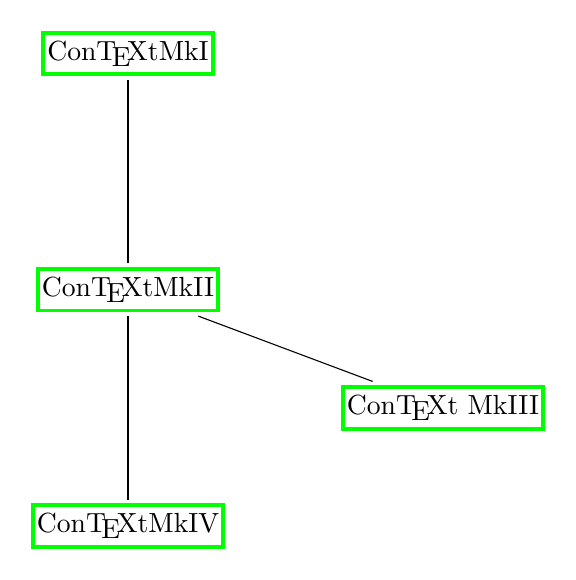
\begin{tikzpicture}
\mynode{mki}{0,0}{Original ConTeXt with Dutch low level interface.}{\ConTeXt MkI};
\mynode{mkii}{0,-3}{ConTeXt with English low level interface. Works with any TeX-engine, like LaTeX: TeX, e-TeX, pdfTeX, Aleph, XeTeX, ...}{\ConTeXt MkII};
\draw (mki) to (mkii);

\mynode{mkiii}{4,-4.5}{Reserved for future use for files supporting XeTeX. Has not been used yet.}{\ConTeXt\ MkIII};
\draw (mkii) to (mkiii);

\mynode{mkiv}{0,-6}{Specially designed for LuaTeX.}{\ConTeXt MkIV};
\draw (mkii) to (mkiv);
\end{tikzpicture}

\newpage
\overviewsection{\TeX's "little" helpers}
\parbox{\textwidth}{This is a small section to mention programs that are very helpful and specially designed to support the work with \TeX.}\vspace{3ex}


\begin{tikzpicture}
\mynode{mki}{0,0}{Very helpful and important tool for creating bibliographies.}{\BibTeX};
\end{tikzpicture}
%%
%% I've chosen to typeset the bibliography "by hand" as to avoid problems regarding formatting. And this way I only need one file.
%%
\clearpage
\part{\color{blue}References}
\newpage
\normalsize
\begin{thebibliography}{10}
\refstepcounter{section}
\label{sec:refs}
\bibitem[{Annotations}()]{}{\quad The references are in order of occurance in the above document. I.\,e. if you want information about Lua\TeX, it will be below e.\,g. $\epsilon$\TeX.}
\vspace{2ex}
\bibitem[{Books}()]{}{\LARGE\textbf{\textsf{Books}}}
\vspace{1ex}
\bibitem[Knuth et~al.(1986)Knuth, Bibby, and Makai]{knuth1986texbook}
D.E. Knuth, D.~Bibby, and I.~Makai.
\newblock \emph{{The \TeX book}}.
\newblock Addison-Wesley Reading, MA, 1986.

\bibitem[Mittelbach et~al.(2004)Mittelbach, Goossens, Braams, Carlisle, Rowley,
  Detig, and Schrod]{mittelbach2004latex}
F.~Mittelbach, M.~Goossens, J.~Braams, D.~Carlisle, C.~Rowley, C.~Detig, and
  J.~Schrod.
\newblock \emph{{The \LaTeX\ companion}}.
\newblock Addison-Wesley, 2004.

\vspace{2ex}
\bibitem[{WebEngines}()]{}{\LARGE\textbf{\textsf{Web Sources}}}
\vspace{1ex}
\bibitem[{OrigDoc}()]{}{\Large\textbf{\textsf{Original Documentation -- Engines}}}
\vspace{1ex}

\bibitem[{ML\TeX\ source}()]{mltex}{ML\TeX\ source (CH file)}
\newblock \url{http://www.tex.ac.uk/tex-archive/systems/generic/mltex/mltex.ch}

\bibitem[{enc\TeX\ page}()]{enctex}
{enc\TeX\ page}
\newblock \url{http://www.olsak.net/enctex.html}

\bibitem[{\NTS\ project page}()]{nts}
{\NTS\ project page}
\newblock \url{http://nts.tug.org}

\bibitem[{$\epsilon\chi$\TeX\ project page}()]{extex}
{$\epsilon\chi$\TeX\ project page}
\newblock \url{http://www.extex.org}

\bibitem[{ee\TeX\ project page}()]{eetex}
{ee\TeX\ project page}
\newblock \url{http://tex.aanhet.net/eetex}

\bibitem[{Lua\TeX\ project page}()]{luatex}
{Lua\TeX\ project page}
\newblock \url{http://www.luatex.org}

\vspace{2ex}
\bibitem[{WebMakro}()]{}{\Large\textbf{\textsf{Original Documentation -- Makro Packages/Formats}}}
\vspace{1ex}
\bibitem[wiki()]{contextgarden}
\ConTeXt\ wiki
\newblock \url{http://wiki.contextgarden.net}

\bibitem[{\LaTeX\ project page}()]{latexproject}
{\LaTeX\ project page}
\newblock \url{http://www.latex-project.org}

\bibitem[{\LaTeX3 project}()]{latexprojectiii}
{\LaTeX3 project}
\newblock \url{http://www.latex-project.org/latex3.html}

\vspace{2ex}
\bibitem[{WebMakro}()]{}{\Large\textbf{\textsf{Overview Articles}}}
\vspace{1ex}
\bibitem[{A Brief History of TeX}()]{mltex}{ Arthur Reutenauer. A Brief History of \TeX.}
\newblock Talk at EuroBacho\TeX\ 2007.\\
\newblock \url{http://www.gust.org.pl/bachotex/EuroBachoTeX2007/presentations/bhot.pdf/view}

\bibitem[{A Brief History of \LaTeX}()]{abriefhistoflatex}
{A Brief History of \LaTeX}
\newblock \url{http://www.xent.com/FoRK-archive/feb98/0307.html}

\bibitem[{omega and aleph}()]{omegaleph}
{Short Article About Omega And Aleph}
\newblock \url{http://www.tex.ac.uk/cgi-bin/texfaq2html?label=omegaleph}
\end{thebibliography}

\clearpage
\part{\color{blue}Text Overview}
\newpage
\setcounter{section}{0}
\end{document}